%convolution result
\par \indent The convolution process returns three haemodynamic response predictions corresponding to neural conditions for parametric gain, parametric loss, and distance from indifference respectively, where are shown in the figures below \ref{fig:convolution}. These haemodynamic responses are crucial to fMRI analysis because fMRI measures haemodynamic responses of the brain to locate neural activities regions.Using the three haemodynamic responses as linear regressors, we obtain three coefficient estimates corresponding to each haemodynamic response for each voxel. The larger the absolute value of a coefficient is, the stronger relationship a haemodynamic response and a voxel have. The figures below show the coefficient estimates for each condition, and each figure contains all slices across the third dimension. The parameter maps show the activation regions in brain corresponding to each task, even though we still need to apply t-test to check the significance level later. 

\begin{figure}[h!]
\centering
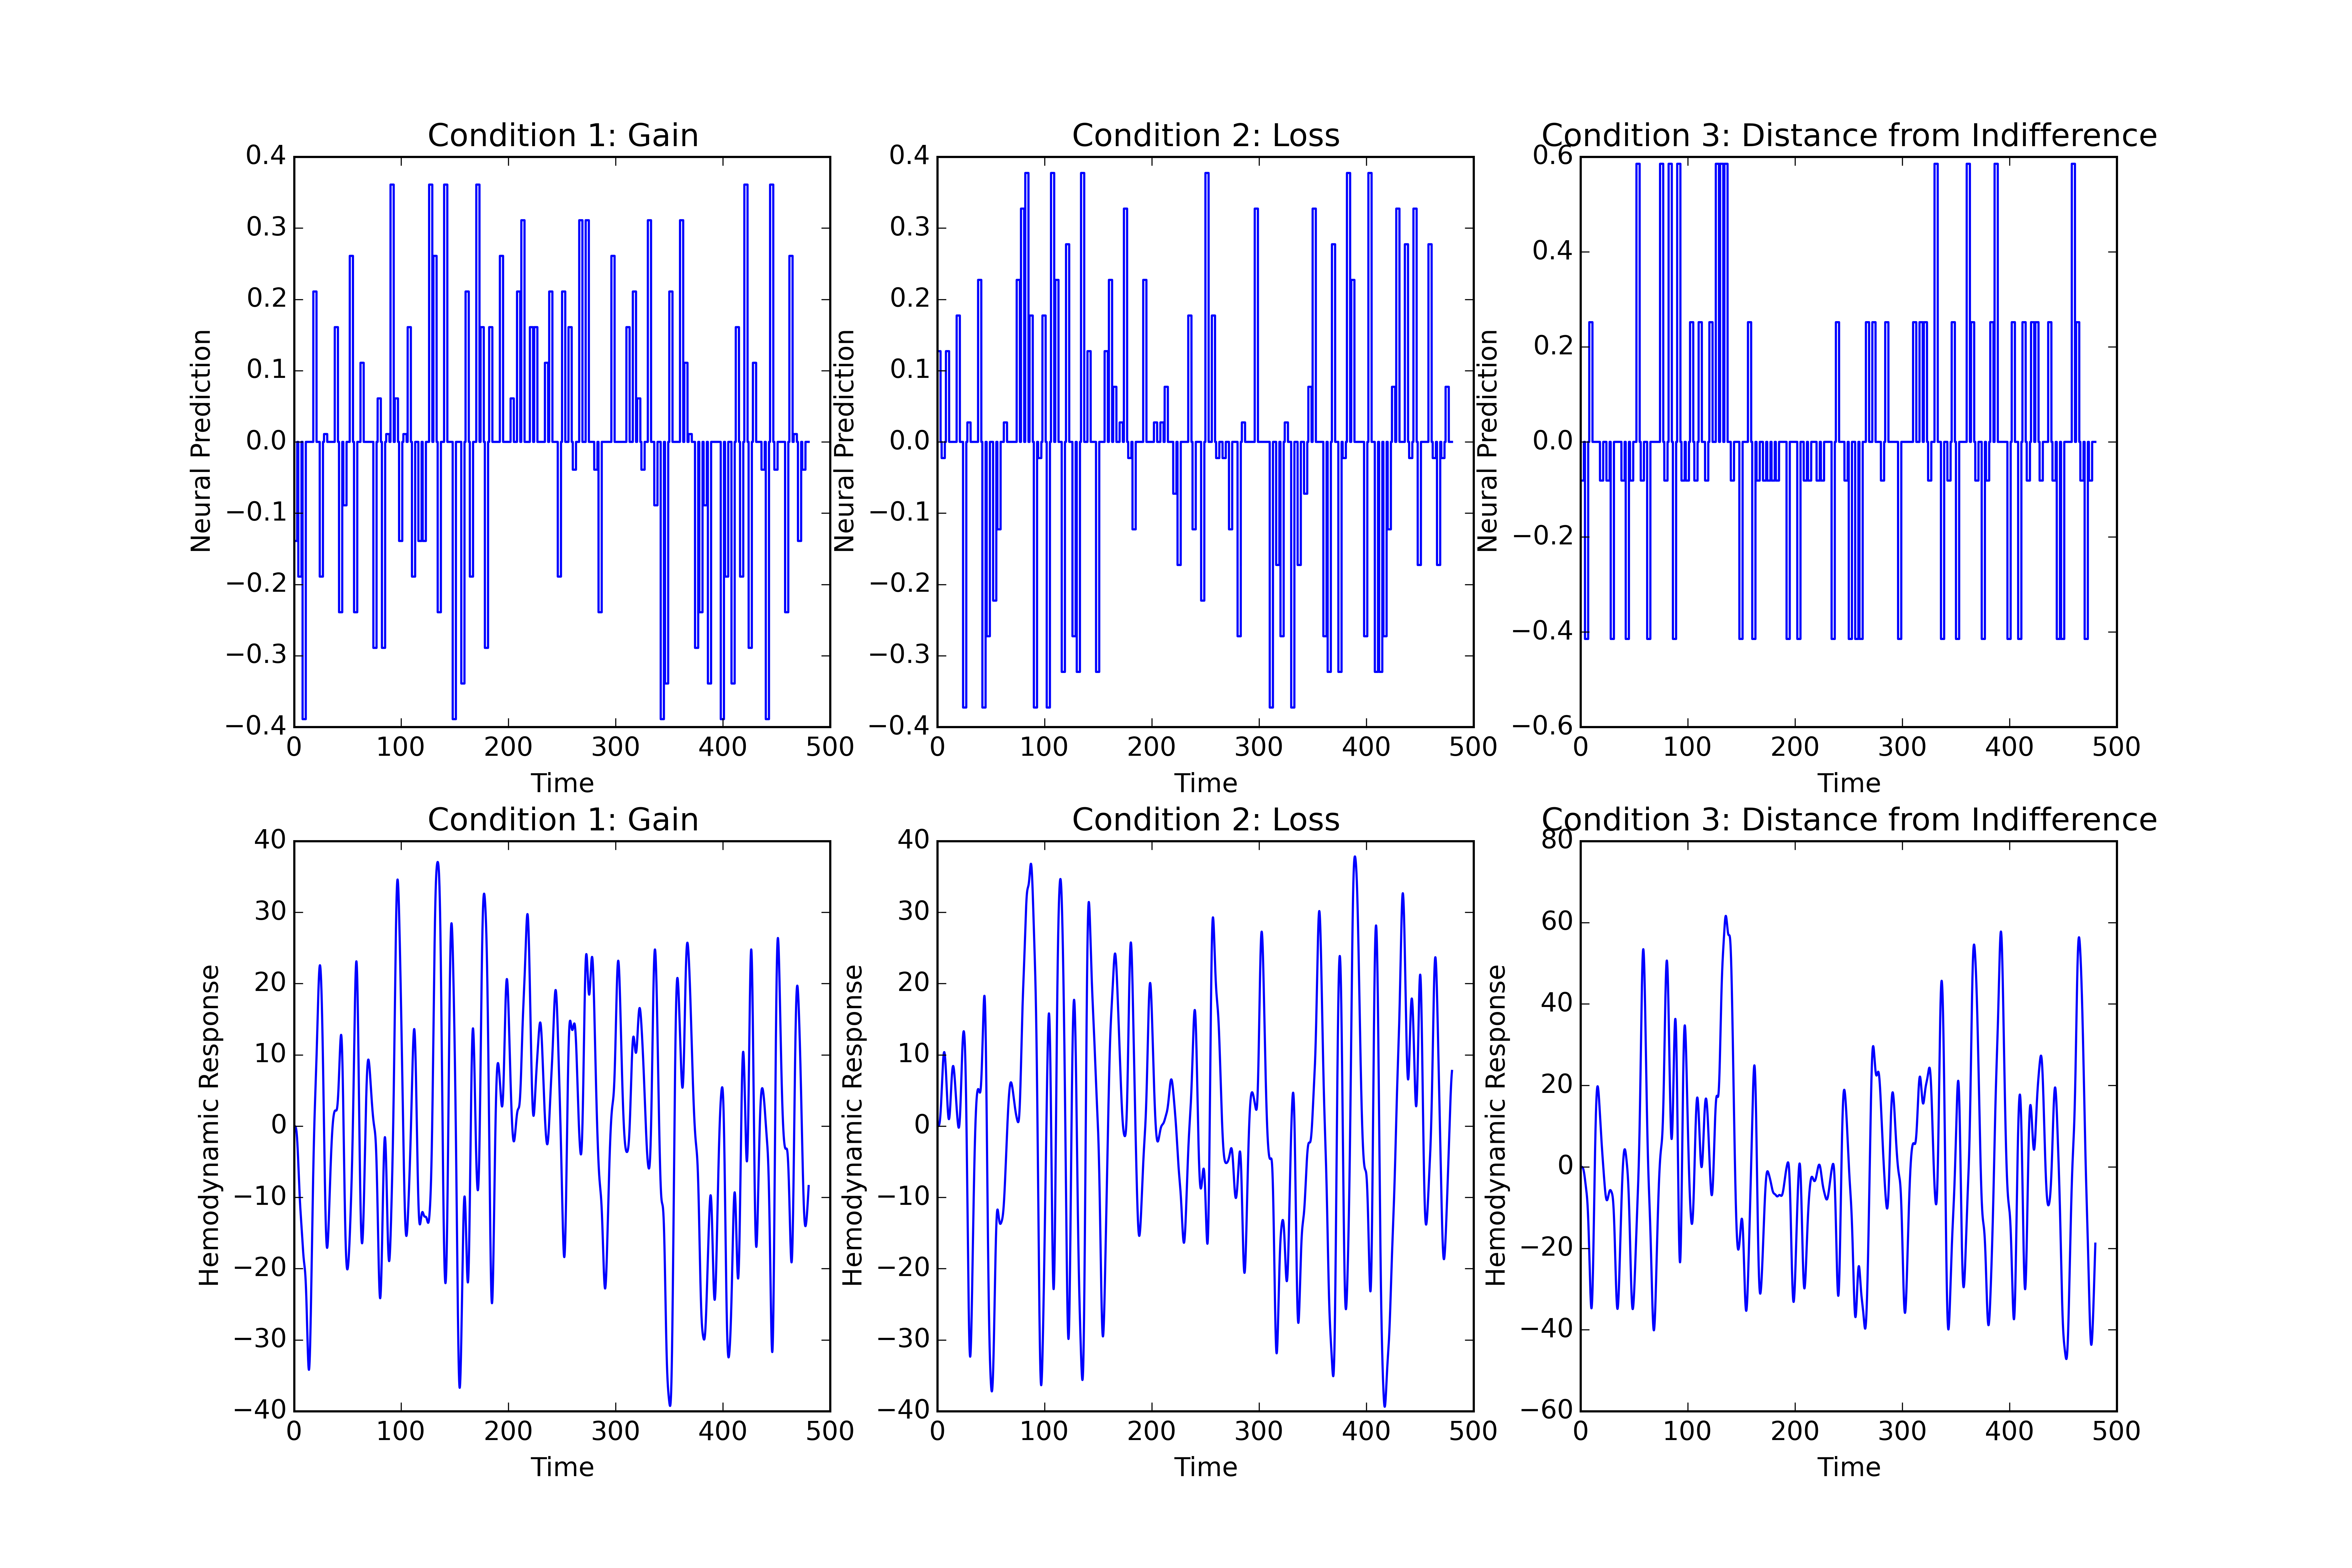
\includegraphics[width=120mm]{images/convolution3cond.png}
\caption{Neural and Haemodynamic Response Predictions for Three Conditions for Subject 1 in Run 1}
\label{fig:convolution}
\end{figure}